\documentclass[12pt, a4paper]{article}

\usepackage[utf8]{inputenc}

% Limit the page margin to only 1 inch.
\usepackage[margin=1in]{geometry}

%Imports biblatex package
\usepackage[
backend=biber,
style=alphabetic
]{biblatex}
\addbibresource{../math-342w.bib}

% Enables the `align' environment.
\usepackage{amsmath}

% Provides useful environments, such as:
% - \begin{proof} ...\end{proof}
\usepackage{amsthm}
\newtheorem{proposition}{Proposition}
\theoremstyle{definition}
\newtheorem*{definition}{Definition}
\newtheorem{theorem}{Theorem}
\newtheorem{corollary}{Corollary}

% Enables using \mathbb{}, for example \mathbb{N} for the set of natural numbers.
\usepackage{amssymb}

% Allows using letters in enumerate list environment. Use, for example:
%\begin{enumerate}[label=(\alph*)]
% ...
%\end{enumerate}
\usepackage[inline]{enumitem}

% Enable importing external graphic files and provides useful commands, like \graphicspath{}
\usepackage{graphicx}
% Images are located in a directory called "images" in the current directory.
\graphicspath{{./images/}}

% Make links look better by default.
% See: https://tex.stackexchange.com/questions/823/remove-ugly-borders-around-clickable-cross-references-and-hyperlinks
\usepackage[hidelinks]{hyperref}
\usepackage{xcolor}
\hypersetup{
	colorlinks,
	linkcolor={red!50!black},
	citecolor={blue!50!black},
	urlcolor={blue!80!black}
}

% Code Listings. Source:
% https://stackoverflow.com/questions/3175105/inserting-code-in-this-latex-document-with-indentation
\usepackage{listings}
\usepackage{color}
\usepackage[most]{tcolorbox}

\definecolor{dkgreen}{rgb}{0,0.6,0}
\definecolor{gray}{rgb}{0.5,0.5,0.5}
\definecolor{mauve}{rgb}{0.58,0,0.82}

\lstset{frame=tb,
	language=Java,
	aboveskip=3mm,
	belowskip=3mm,
	showstringspaces=false,
	columns=flexible,
	basicstyle={\small\ttfamily},
	numbers=none,
	numberstyle=\tiny\color{gray},
	keywordstyle=\color{blue},
	commentstyle=\color{dkgreen},
	stringstyle=\color{mauve},
	breaklines=true,
	breakatwhitespace=true,
	tabsize=3
}

\newcommand{\prob}{\text{P}}
%\newcommand{\complement}{\mathsf{c}}
\title{Lecture 9: MATH 342W: Introduction to Data Science and Machine Learning}
\author{Sergio E. Garcia Tapia\thanks{Based on lectures of Dr. Adam Kapelner at Queens College.
See also the \href{https://github.com/kapelner/QC_MATH_342W_Spring_2025}{course GitHub page}.}}
\date{February 27, 2025 (last updated \today)}

\begin{document}
	\maketitle
	\section*{Recap}
	Last time, we saw that $\hat{\mathbf{y}}$ is the projection of $\mathbf{y}$ onto
	the column space of $X$ (see Figure~\ref{fig:prediction-space}). We can express
	this as
	\begin{figure}
		\centering
		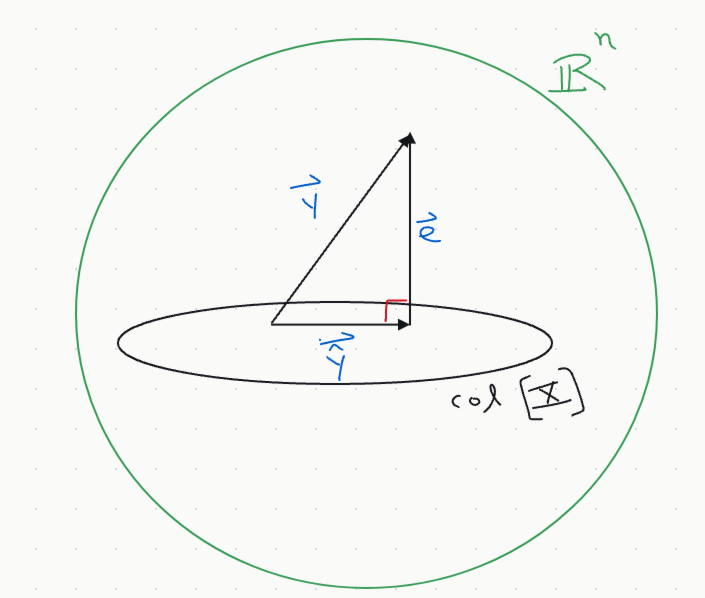
\includegraphics[width=0.5\textwidth]{prediction-orthogonal-projection}
		\caption{The prediction $\hat{\mathbf{y}}$ viewed as an orthogonal
			projection of the response vector $\mathbf{y}$ onto the column space of $X$.}
		\label{fig:prediction-space}
	\end{figure}
	\begin{align*}
		\hat{\mathbf{y}}& = \underset{co\ell[X]}{\text{proj}(\mathbf{y})}\\
		&=X(X^\top X)^{-1}X^\top \mathbf{y}\\
		&=H\mathbf{y}
	\end{align*}
	where $H$ is the Hat matrix. What is $\underset{co\ell[X]}{\text{proj}}(\hat{\mathbf{y}})$?
	That is, what happens if we project $\hat{\mathbf{y}}$ onto the column space of $X$?
	Intuitively, it should be $\hat{\mathbf{y}}$, because $\hat{\mathbf{y}}$ is what
	we get from projecting $\mathbf{y}$ onto the column space of $X$, so
	$\hat{\mathbf{y}}$ is already in $co\ell[X]$. If this is the case,
	then we expect the following equalities to hold:
	\begin{align*}
		\underset{co\ell[X]}{\text{proj}}(\hat{\mathbf{y}})
		&=\underset{co\ell[X]}{\text{proj}}(\underset{co\ell[X]}{\text{proj}(\mathbf{y})})\\
		&=H(H\mathbf{y})\\
		&=H^2\mathbf{y}\\
		&=H\mathbf{y}\\
		&=\hat{\mathbf{y}}
	\end{align*}
	Therefore, we conjecture that $H\cdot H=H$. Before we explore this idea, let's consider
	the null model again.
	\section*{The Null Model in Multivariate Regression}
	In the null model $g_0$, we do not take any features into account, so $p=0$. In this case,
	we expect $g_0$ to predict $\bar{y}$ for all inputs, as we saw when we first tackled OLS.
	Since $p=0$ and there are $n$ responses, the matrix $X$ is of dimension $n\times (p+1)$ or
	$n\times 1$, where the first (and only) column has all $1$'s, like so:
	\begin{align*}
		X=\begin{bmatrix}
			1\\
			1\\
			\vdots\\
			1
		\end{bmatrix}
		=\vec{\mathbf{1}}_n
	\end{align*}
	Now let's compute $H$:
	\begin{align*}
		H&=X(X^\top X)^{-1}X^\top\\
		&=\vec{\mathbf{1}}_n(\vec{\mathbf{1}}_n^\top \vec{\mathbf{1}}_n)^{-1} \vec{\mathbf{1}}_n^\top\\
		&=\vec{\mathbf{1}}_n\left(n\right)^{-1}\vec{\mathbf{1}}_n
		\tag{$\vec{\mathbf{1}}_n^\top \vec{\mathbf{1}}_n=n$}\\
		&=\frac{1}{n}\vec{\mathbf{1}}_n \vec{\mathbf{1}}_n^\top
	\end{align*}
	Notice that since $\vec{\mathbf{1}}_n$ is $n\times 1$ and $\vec{\mathbf{1}}_n^\top$ is $1\times n$,
	the result of $\vec{\mathbf{1}}_n \vec{\mathbf{1}}_n^\top$ is an $n\times n$ matrix. The product
	$\vec{\mathbf{1}}_n \vec{\mathbf{1}}_n^\top$ is known as an \textit{outer product}. It's easy to
	verify that the resulting matrix will have all $1$'s, so
	\begin{align*}
		H &=\frac{1}{n}\vec{\mathbf{1}}_n \vec{\mathbf{1}}_n^\top\\
		&=\frac{1}{n}\begin{bmatrix}
			1 & \cdots & 1\\
			\vdots & \cdots & \vdots\\
			1 & \cdots & 1
		\end{bmatrix}
		\tag{The matrix is $n$ by $n$.}\\
		&=\begin{bmatrix}
			\frac{1}{n} & \cdots & \frac{1}{n}\\
			\vdots & \cdots & \vdots\\
			\frac{1}{n} & \cdots & \frac{1}{n}
		\end{bmatrix}
	\end{align*}
	In particular, since every column is a scalar multiple of the first, the rank
	of this matrix is $1$, i.e., $\text{rank}(H)=1$, which is the number of columns
	in $X$ (indeed, we saw last time that $\text{rank}(H)=p+1$). Now we can
	compute the prediction:
	\begin{align*}
		\hat{\mathbf{y}} = H\mathbf{y}
		=\begin{bmatrix}
			\frac{1}{n} & \cdots & \frac{1}{n}\\
			\vdots & \cdots & \vdots\\
			\frac{1}{n} & \cdots & \frac{1}{n}
		\end{bmatrix}\mathbf{y}
		=\begin{bmatrix}
			\frac{1}{n}\sum_{i=1}^{n}y_i\\
			\vdots\\
			\frac{1}{n}\sum_{i=1}^{n}y_i
		\end{bmatrix}
		=\bar{y}\cdot  \vec{\mathbf{1}}_n
	\end{align*}
	Hence, all $n$ responses are predicted to be $\overline{y}$.
	\section*{Properties of Orthogonal Projections}
	We have mentioned that $H$ is an orthogonal projection. We will formally define what
	orthogonal projections are, and prove some useful properties that they satisfy.
	\begin{tcolorbox}[breakable]
		\begin{definition}
			A matrix $P$ is an \textbf{orthogonal projection matrix} if and only if
			$\forall_{\mathbf{v}, \mathbf{w}\in\mathbf{R}^n}$, we have
			\begin{align*}
				(\mathbf{v}-P\mathbf{v})^\top (P\mathbf{w})=0
			\end{align*}
		\end{definition}
	\end{tcolorbox}
	That definition says that $P\mathbf{w}$ and $(\mathbf{v}-P\mathbf{v})$ are orthogonal
	for every $\mathbf{v},\mathbf{w}\in\mathbb{R}^n$.
	\begin{tcolorbox}[breakable]
		\begin{theorem}
			\label{thm:orthogonal-proj-matrix}
			A matrix $P$ is an orthogonal projection if and only if the following two
			are both satisfied:
			\begin{enumerate}[label=(\roman*)]
				\item \textbf{Symmetric}: $P^\top=P$.
				\item \textbf{Idempotent}: $P^2=P$ (it squares to itself).
			\end{enumerate}
		\end{theorem}
		\begin{proof}
			We will prove the $if$ direction ($\impliedby$), and leave $\implies$ as an exercise.
			Thus, we are assuming that $P^\top=P$ and $P^2=P$. We have to show that it satisfies
			the definition of an orthogonal projection. Let $\mathbf{v},\mathbf{w}\in \mathbb{R}^n$. Then
			\begin{align*}
				(\mathbf{v}-P\mathbf{v})^\top P\mathbf{w}
				&= (\mathbf{v}^\top - \mathbf{v}^\top P^\top)P\mathbf{w}\\
				&=\mathbf{v}^\top P\mathbf{w}-\mathbf{v}^\top P^\top\cdot P\mathbf{w}\\
				&=\mathbf{v}^\top P\mathbf{w}-\mathbf{v}^\top P \cdot P\mathbf{w}
				\tag{Symmetry: $P^\top=P$}\\
				&=\mathbf{v}^\top P\mathbf{w}-\mathbf{v}^\top P^2\mathbf{w}\\
				&=\mathbf{v^\top}P\mathbf{w}-\mathbf{v}^\top P\mathbf{w}
				\tag{Idempotency: $P^2=P$}\\
				&=0
			\end{align*}
		\end{proof}
	\end{tcolorbox}
	Let's verify $H$ satisfies the conditions of Theorem~\ref{thm:orthogonal-proj-matrix}.
	First, we will check that $H^\top=H$:
	\begin{align*}
		H^\top&=\left(X(X^\top X)^{-1}X^\top\right)^\top\\
		&=(X^\top)^\top [(X^\top X)^{-1}]^\top X^\top
		\tag{by $(AB)^\top=B^\top A^\top$}\\
		&=X[(X^\top X)^\top]^{-1}X^\top
		\tag{by $(A^{-1})^\top = (A^\top)^{-1}$}\\
		&=X[X^\top X]^{-1}X^\top
		\tag{since $(X^\top X)^\top = X^\top X$}\\
		&=H
	\end{align*}
	Next, let's check that $H^2=H$:
	\begin{align*}
		H^2&=H\cdot H\\
		&=(X(X^\top X)^{-1}X^\top)(X(X^\top X)^{-1}X^\top)\\
		&=X(X^\top X)^{-1}\underbrace{[(X^\top X)(X^\top X)^{-1}]}_{I_{p+1}}X^\top\\
		&=X(X^\top X)^{-1}X^\top\\
		&=H
	\end{align*}
	Thus, $H$ is indeed an orthogonal projection matrix.
	\section*{Orthogonal Projection onto Residual Space}
	Now let's revisit an idea we mentioned last time, in which we said that $I_n-H$ is
	also an orthogonal projection matrix. This time, however, it is a projection
	onto the residual space (see Figure~\ref{fig:residual-space}).
	\begin{figure}
		\centering
		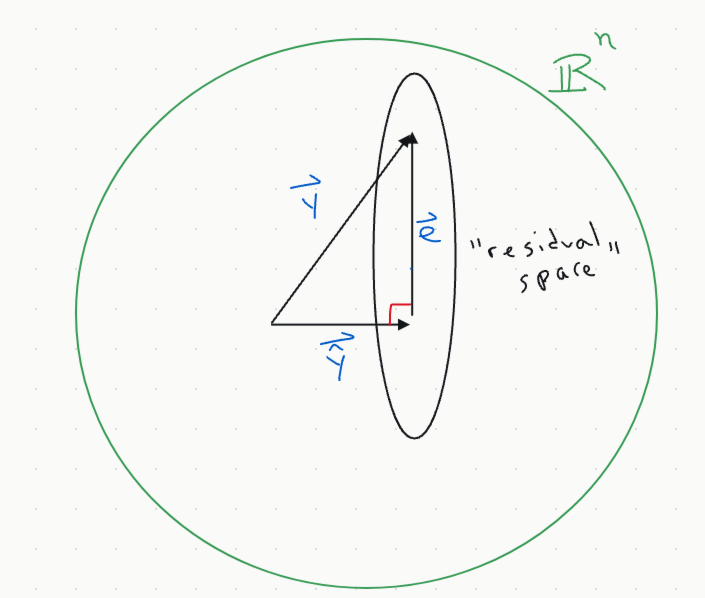
\includegraphics[width=0.5\textwidth]{residual-space}
		\caption{The residual $\mathbf{e}$ viewed as an orthogonal
			projection of the response vector $\mathbf{y}$ onto the ``residual space".}
		\label{fig:residual-space}
	\end{figure}
	To justify this, we must argue as in the case for $H$, by showing $I_n-H$ satisfies
	both conditions of Theorem~\ref{thm:orthogonal-proj-matrix}. We will leverage
	the idempotency and symmetry of $H$:
	\begin{enumerate}[label=(\roman*)]
		\item \textbf{Symmetric}: We must show $(I_n-H)^\top=(I_n-H)$:
		\begin{align*}
			(I_n-H)^\top &=I_n^\top -H^\top=I_n-H
		\end{align*}
		Note that the identify matrix is indeed symmetric, and we've used the fact that $H$ is, too.
		\item \textbf{Idempotent}: We must show $(I_n-H)^2=(I_n-H)$:
		\begin{align*}
			(I_n-H)^2 &= (I_n-H)(I_n-H)\\
			&=I_n\cdot I_n - I_n\cdot H-H\cdot I_n+H^2\\
			&=I_n -H-H+H
			\tag{$H$ is idempotent}\\
			&=I_n-H
		\end{align*}
	\end{enumerate}
	\section*{$SSR$, $R^2$, and Geometric Interpretations}
	Consider again Figure~\ref{fig:prediction-space}. Since $\hat{\mathbf{y}}$ and
	$\mathbf{e}$ are orthogonal, note that Pythagorean's Theorem says that
	\begin{align*}
		\|\mathbf{y}\|^2 &= \|\hat{\mathbf{y}}\|^2 + \|\mathbf{e}\|^2
	\end{align*}
	See Figure~\ref{fig:pyth-thm-y-yhat-e}.
	\begin{figure}
		\centering
		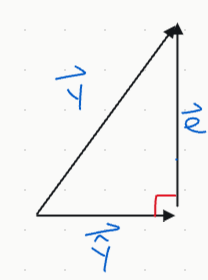
\includegraphics[width=0.15\textwidth]{pythagorean-theorem-y-yhat-e}
		\caption{Orthogonal decomposition of response $\mathbf{y}$ into prediction $\hat{\mathbf{y}}$ and
		residual error $\mathbf{e}$.}
		\label{fig:pyth-thm-y-yhat-e}
	\end{figure}
	We will use this geometric intuition in a moment.
	Let's attempt to come up with a fit for $\mathbf{y}-\bar{y}\cdot \vec{\mathbf{1}_n}$
	(referred to as the \textit{mean-control response}) by projecting it onto $co\ell[X]$:
	\begin{align*}
		\underset{co\ell[X]}{\text{proj}}(\mathbf{y}-\bar{y}\cdot \vec{\mathbf{1}}_n)
		&=H(\mathbf{y}-\bar{y}\cdot \vec{\mathbf{1}}_n)\\
		&=H\mathbf{y}-\bar{y}\cdot H\vec{\mathbf{1}}_n\\
		&=\hat{\mathbf{y}}-\bar{y} \cdot\vec{\mathbf{1}}_n
		\tag{$\vec{\mathbf{1}}_n\in co\ell[X]\implies \vec{\mathbf{1}}_n\in co\ell[H]$}
	\end{align*}
	Now
	\begin{align*}
		(\mathbf{y}-\bar{y}\cdot\vec{\mathbf{1}}_n) - (\hat{\mathbf{y}} - \bar{y}\cdot\vec{\mathbf{1}}_n)
		&=\mathbf{y}-\hat{\mathbf{y}}=\mathbf{e}
	\end{align*}
	In particular, the two vectors being subtracted above are orthogonal
	(see Figure~\ref{fig:pyth-thm-mean-control-response}).
	\begin{figure}
		\centering
		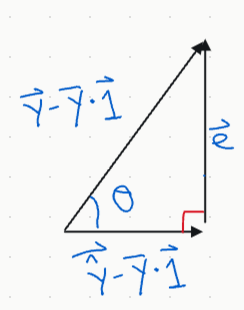
\includegraphics[width=0.2\textwidth]{pythagorean-theorem-mean-control-response}
		\caption{Orthogonal decomposition of mean-control response $\mathbf{y}-\bar{y}\cdot \vec{\mathbf{1}}_n$
		into $\hat{\mathbf{y}}-\bar{y}\cdot \vec{\mathbf{1}}_n$ and residual error $\mathbf{e}$.}
		\label{fig:pyth-thm-mean-control-response}
	\end{figure}
	Therefore, by Pythagorean's Theorem
	\begin{align}
		\|\mathbf{y} - \bar{y}\cdot \vec{\mathbf{1}}_n\|^2
		&= \|\hat{\mathbf{y}}-\bar{y}\cdot \vec{\mathbf{1}}_n\|^2
		+ \|\mathbf{e}\|^2\nonumber\\
		\sum_{i=1}^{n}(y_i-\bar{y})^2 &= \sum_{i=1}^{n}(\hat{y}_i-\bar{y})^2
		+\sum_{i=1}^{n}e_i^2\nonumber\\
		SST &= SSR + SSE\label{eqn:sst=ssr+sse}
	\end{align}
	\begin{tcolorbox}
		\begin{definition}
			Given a $n$ real numbers $(y_i)_{i=1}^{n}$ with mean $\bar{y}$ and associated
			predictions $(\hat{y}_i)_{i=1}^{n}$, the $SSR$ is given by
			\begin{align*}
				SSR = \sum_{i=1}^{n}(\hat{y}_i-\bar{y})^2
			\end{align*}
		\end{definition}
	\end{tcolorbox}
	Using trigonometry, we can see that
	\begin{align*}
		\cos^2\theta &=
		\frac{\|\hat{\mathbf{y}} - \bar{y}\cdot \vec{\mathbf{1}}_n\|^2}{\|\mathbf{y} - \bar{y}\cdot \vec{\mathbf{1}}_n\|^2}\\
		&=\frac{SSR}{SST}
		\tag{by Equation~\ref{eqn:sst=ssr+sse}}\\
		&=\frac{SST-SSE}{SST}\\
		&=1-\frac{SSE}{SST}\\
		&=R^2
	\end{align*}
	Since $\cos^2\theta\in [0, 1]$, we see that $R^2\in [0, 1]$.
	Let's think about what this means. If your projection $\hat{\mathbf{y}}$ is close
	to the response vector $\mathbf{y}$, then the angle between them is small. On the
	other hand, if $\theta=90^\circ$, then there is no fit. In the latter case,
	$\hat{\mathbf{y}}-\bar{y}\cdot \vec{\mathbf{1}}$ is the zero vector, so
	$\hat{\mathbf{y}}=\bar{y}\vec{\mathbf{1}}_n$, and hence we did not do better than the null
	model $g_0$.
	\begin{figure}
		\centering
		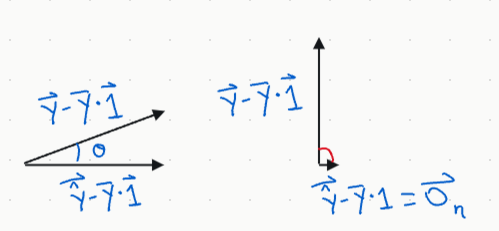
\includegraphics[width=0.5\textwidth]{mean-control-response-angle}
		\caption{Depictions related to mean-control response in two cases: (i) high $R^2$, and 
			(ii) $\theta=90^\circ$, where we do not beat $g_0$.}
		\label{fig:control-response-angle}
	\end{figure}
	\section*{Reviewing Ignorance Error}
	Recall that ignorance error comes from the fact that the features (the $x$'s) do not give
	sufficient information about the true drivers (the $z$'s). We mentioned that a way to
	address that is by adding more features (increase $p$).
	
	Let $X'=[X \mid \mathbf{x}_{\cdot \text{new}}]$, where we append a new column
	corresponding to a new feature that we measure. Then we expect that the error
	will decrease, and hence the angle between $\mathbf{y}$ and $\hat{\mathbf{y}}$
	correspondingly decreases (see Figure~\ref{fig:add-new-feature}).
	\begin{figure}
		\centering
		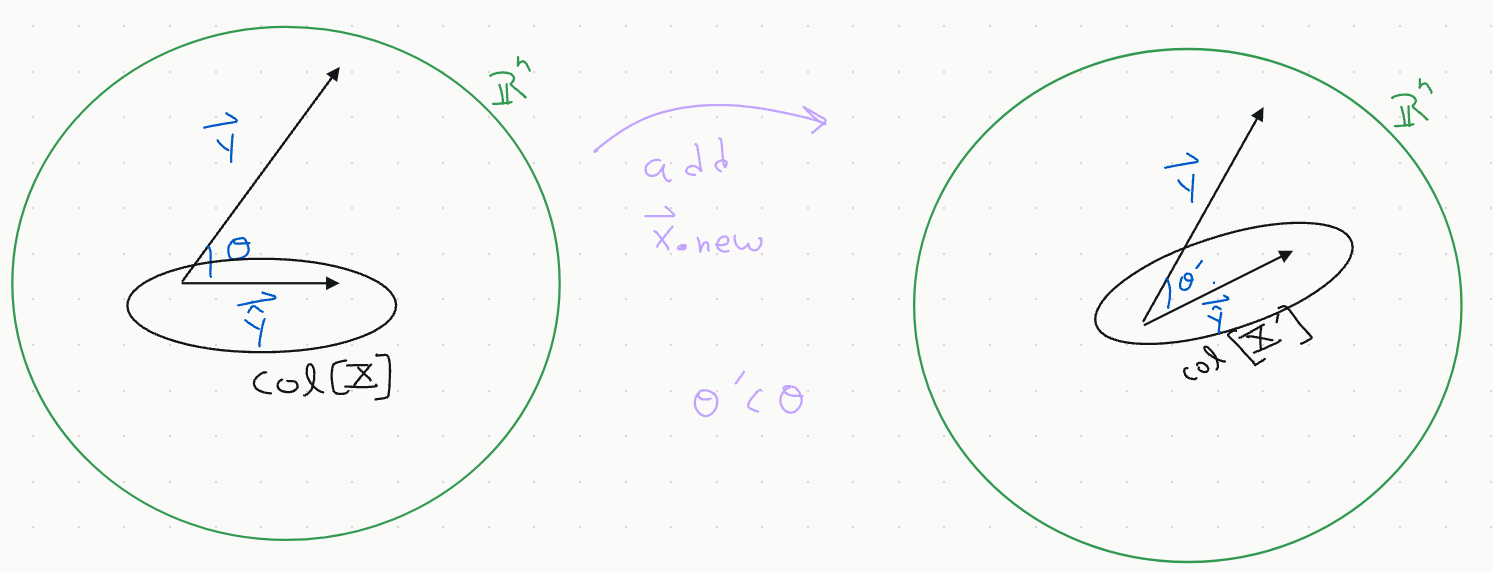
\includegraphics[width=1.0\textwidth]{adding-new-feature}
		\caption{Adding a new feature to $X$. We expect $\theta$ to decrease.}
		\label{fig:add-new-feature}
	\end{figure}
	In the case where $p=1$, we have $X=[\vec{\mathbf{1}} \mid \mathbf{x}_{\cdot, 1}]$,
	so $co\ell[X]$ is a 2-dimensional plane. See Figure~\ref{fig:one-feature}.
	\begin{figure}
		\centering
		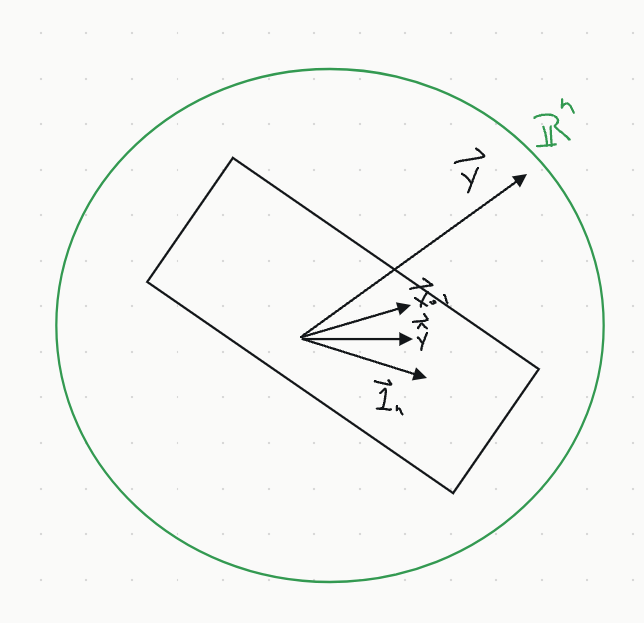
\includegraphics[width=0.7\textwidth]{one-feature}
		\caption{Illustration of least square when using $1$ feature.
		Depicted is the portion of $\mathbf{y}$ along $\mathbf{x}_{\cdot 1}$
		(the weight $b_1$) and the portion of $\mathbf{y}$ along $\vec{\mathbf{1}}_n$
		(the intercept $b_0$)}
		\label{fig:one-feature}
	\end{figure}
	\section*{Eigenvectors and Eigenvalues of $H$}
	The following material is outside the scope of this class, in the sense that you are not
	required to know it. Nevertheless, we will explore the concepts.
	
	Recall that $X$ has a column of $1$'s and $p$ columns of features:
	\begin{align*}
		X = \begin{bmatrix}
			\vec{\mathbf{1}}_n & \mathbf{x}_{\cdot, 1} & \cdots & \mathbf{x}_{\cdot, p}
		\end{bmatrix}
	\end{align*}
	In particular, the columns of $X$ are clearly in the column space of $X$.
	Recall that $H$ is the orthogonal projection matrix onto the column space of $X$.
	This means that
	\begin{align*}
		H\vec{\mathbf{1}}_n=\vec{\mathbf{1}}_n,\quad
		H\mathbf{x}_{\cdot, 1} = \mathbf{x}_{\cdot, 1},\quad
		\cdots,\quad
		H\mathbf{x}_{\cdot, p} = \mathbf{x}_{\cdot, p}
	\end{align*}
	One simple way to verify this is as follows:
	\begin{align*}
		HX &= (X(X^\top X)^{-1}X^\top)X\\
		&=X[(X^\top X)^{-1}(X^\top X)]\\
		&=X\cdot I_{p+1}\\
		&=X
	\end{align*}
	We conclude that $\lambda=1$ is an eigenvalue of $H$, and the eigenspace associated
	with $\lambda=1$ is spanned by $\mathbf{1},\mathbf{x}_{\cdot, 1},\ldots,\mathbf{x}_{\cdot, p}$.
	Since $H$ is symmetric (i.e., self-adjoint), the spectral theorem guarantees that it has an
	eigendecomposition (\textit{diagonalization}) (see \cite{axler}). Thus, we can write
	\begin{align*}
		H = P^{-1}DP
	\end{align*}
	where
	\begin{align*}
		P=\begin{bmatrix}
			\mathbf{v}_1 & \mathbf{v}_2 & \cdots & \mathbf{v}_n
		\end{bmatrix},
		\quad
		D=\begin{bmatrix}
			\lambda_1 &0 & \cdots & 0\\
			0 & \lambda_2 & \cdots & 0\\
			\vdots & \cdots & \ddots & \vdots\\
			0 & \cdots & 0 & \lambda_n
		\end{bmatrix}
	\end{align*}
	Here, $D$ is a diagonal matrix consisting of the eigenvalues of $H$, and
	$P$ is an invertible matrix whose columns are the eigenvectors of $H$.
	We have already argued that
	\begin{align*}
		\mathbf{v}_1=\mathbf{1}_n,\quad
		\mathbf{v}_2=\mathbf{x}_{\cdot, 1},\quad
		\ldots,\quad
		\mathbf{v}_{p+1}=\mathbf{x}_{\cdot, p}.\\
		\lambda_1=\lambda_2=\cdots=\lambda_{p+1}=1
	\end{align*}
	What about the remaining $n-(p+1)$ eigenvectors? Note that if a vector belongs to
	$co\ell[X]^\perp$ (the orthogonal complement of $co\ell[X]$ or equivalently the residual space),
	then $H$ maps it to $0$. Therefore, the remaining $n-(p+1)$ eigenvalues of $H$ are all zero,
	and the eigenvectors associated with the $0$ eigenvalue span $co\ell[X]^\perp$.
	\begin{align*}
		P&=\begin{bmatrix}
			\vec{\mathbf{1}} & \mathbf{x}_{\cdot, 1} & \cdots & \mathbf{x}_{\cdot, p}
			& \mathbf{x}_{\perp, \cdot, 1} & \cdots & \mathbf{x}_{\perp, \cdot, n-(p+1)}
		\end{bmatrix}\\
		D&=\begin{bmatrix}
			1 &0 & \cdots & \cdots &\cdots & 0\\
			0 & \ddots & \ddots & \vdots & \vdots & \vdots\\
			\vdots & \ddots & 1 & \ddots &\vdots & \vdots\\
			\vdots & \vdots & \ddots & 0 & \ddots & \vdots\\
			\vdots & \cdots & \cdots &\ddots  & \ddots & \vdots\\
			0 & \cdots & \cdots & \cdots & \ddots & 0
		\end{bmatrix}
	\end{align*}
	One last fact is related to the trace of $H$. Recall this is the sum of the diagonal
	entries. We'll leverage the diagonalization:
	\begin{align*}
		\sum_{i=1}^{n}h_{i,i}&=\text{tr}[H]\\
		&=\text{tr}[P^{-1}DP]\\
		&=\text{tr}[PP^{-1}D]
		\tag{$\text{tr}[ABC]=\text{tr}[CAB]=\text{tr}[BCA]$}\\
		&=\text{tr}[D]\\
		&=p+1\\
		&=\text{rank}(X)
	\end{align*}
	\pagebreak
	\printbibliography
\end{document}